\documentclass[a4paper]{article}

\usepackage[english]{babel}
\usepackage[latin1]{inputenc}
\usepackage{amssymb}
\usepackage{framed}
\usepackage{graphicx}
\usepackage{subcaption}
\usepackage{float}

\setlength{\parindent}{0pt}
\setlength{\parskip}{3ex}

\begin{document}

\begin{center}
  {\large Artificial Neural Networks and Deep Architectures, DD2437}\\
  \vspace{7mm}
  {\huge Short report on lab assignment 3\\[1ex]}
  {\Large Hopfield networks}\\
  \vspace{8mm}
  {\Large Etienne Jodry, Frano Rajic, Ivan Stresec\\}
  \vspace{4mm}
  {\large September 27, 2020\\}
\end{center}

\section{Main objectives and scope of the assignment}

Our major goals in the assignment were:
\begin{itemize}
\item implementation and testing of Hopfield networks
\item demonstrate how auto-associatives networks can be used to do pattern completion and noise reduction
\item analysing attractor dynamics of Hopfield networks
\item investigating the storage capacity and explore features that help increase it in associative memories
\end{itemize}

We construct an auto-associative memory of the Hopfield type, and explore its capabilities, capacity and limitations. We study the networks dynamics and analyse its origins.

\section{Methods}

We have used Python 3.8 with some of its built-in libraries along with Matplotlib and NumPy libraries for all of our experiments. We also often utilized Jupyter Notebooks and Google Sheets for result visualization and analysis.

\section{Results and discussion}

We modeled a configurable Hopfield network model that was used for solving all of the following tasks. The model uses self connections by default. In all of the following tasks, self connections are used unless otherwise stated.

\subsection{Convergence and attractors}
To start using Hopfield networks, we used a network with 8 neurons and using the Hebbian learning rule stored three 8-dimensional patterns in it. We used batch learning for this task. All three patterns were, as expected, stable states, i.e. attractors.

When testing the network using patterns with a 1-bit mistake, and two 2-bit mistakes. The network converged to a stored pattern for the 1-bit mistake and one of the 2-bit mistake patterns, but didn't converge to a stored pattern for the second pattern with the 2-bit mistake.

Testing all possibilities, we found that the network has 14 attractors. When using very distorted stored patterns the convergence often leads to another attractor, i.e. fails to complete the distorted pattern.

\subsection{Sequential Update}
For this subassignment we loaded patterns from \texttt{pict.dat} and created a 1024-dimensional network to handle them. 

Our network successfully learned patterns/pictures p1, p2, and p3. We could observe all of them were stable states, an update starting from one of those pictures would never produce any change in neuron activity.

Giving the network pattern p10, which is a degraded pattern p1, would converge to p1, but giving the network pattern p11, a mix of p2 or p3, would converge to a stable state, but that state was neither p2 or p3. If using sequential updating (adding a stochastic effect to updating) the network would sometimes converges to p3.

Giving the network a random state and using the sequential updating rule leads to convergence to one of the attractors (stable states). In Figure \ref{fig:sequential_convergence} we can see the process of convergence to a stable state.

\begin{figure}[h]
    \centering
    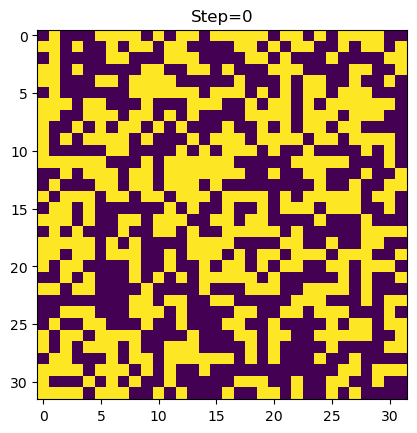
\includegraphics[width=.24\linewidth]{img/seq_1.png}
    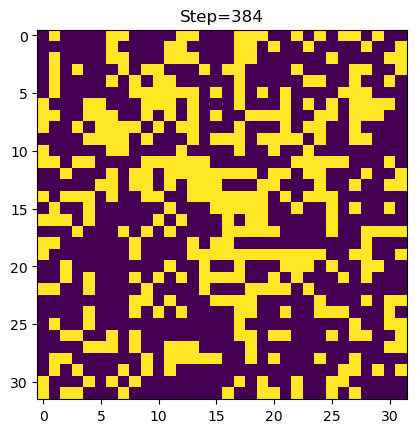
\includegraphics[width=.24\linewidth]{img/seq_2.png}
    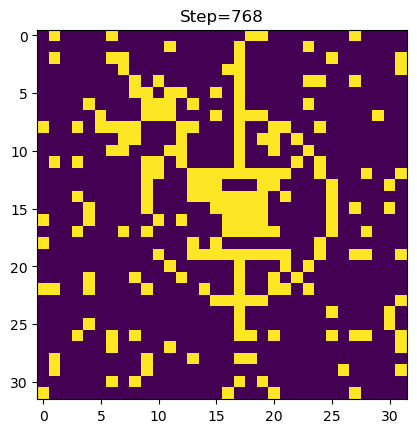
\includegraphics[width=.24\linewidth]{img/seq_3.png}
    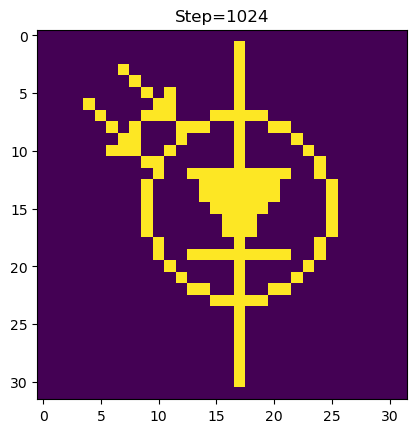
\includegraphics[width=.24\linewidth]{img/seq_4.png}
    \caption{Convergence process using the sequential updating rule}
    \label{fig:sequential_convergence}
\end{figure}

\subsection{Energy}
Our 3 first attractors are the learnt patterns, then we sampled $1000$ randomly generated patterns and executed the update rule until convergence for each of them, to find new attractors.
\begin{figure}[h]
    \centering
    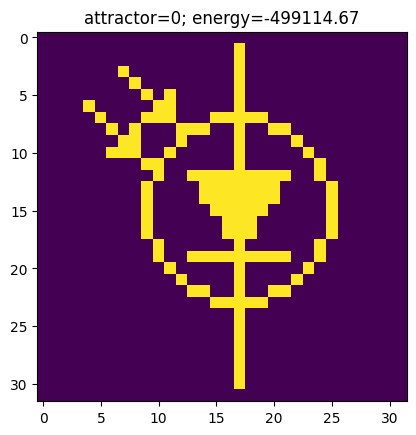
\includegraphics[width=.24\linewidth]{img/attractor=0.png}
    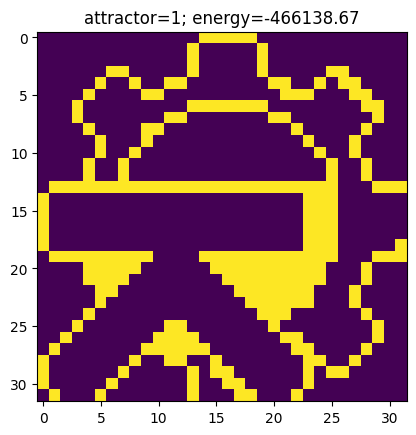
\includegraphics[width=.24\linewidth]{img/attractor=1.png}
    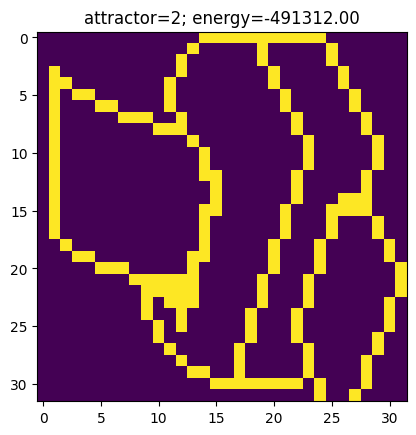
\includegraphics[width=.24\linewidth]{img/attractor=2.png}
    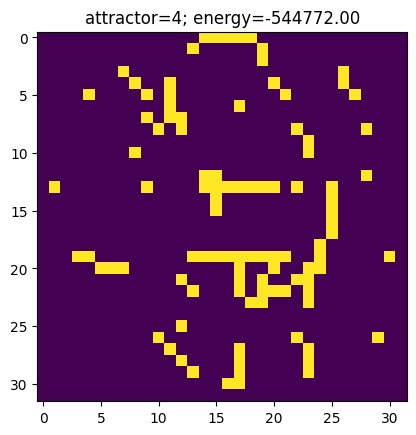
\includegraphics[width=.24\linewidth]{img/attractor=4.png}\\
    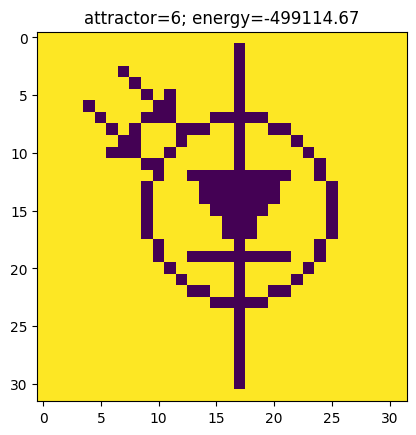
\includegraphics[width=.24\linewidth]{img/attractor=6.png}
    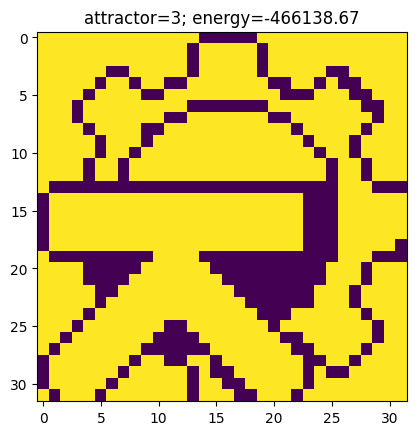
\includegraphics[width=.24\linewidth]{img/attractor=3.png}
    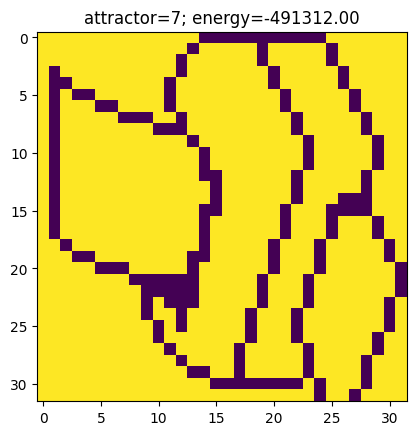
\includegraphics[width=.24\linewidth]{img/attractor=7.png}
    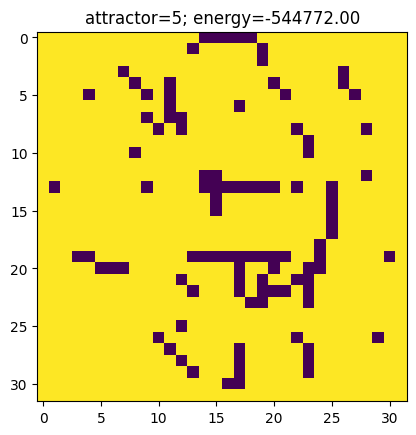
\includegraphics[width=.24\linewidth]{img/attractor=5.png}
    \caption{Attractors and their energies, for network that learnt pictures 1, 2, 3. Learn patterns are the first three images in first row. Other images show spurious states.}
    \label{fig:nrg_att}
\end{figure}

We found 8 attractors in total, it is interesting to note that each attractor has it's "negative" counterpart of same energy. The learnt patterns and their counterparts have roughly an energy of $-5 * 10^5$ each. The global minimum is the newly found attractor that we did not learn (last column on fig \ref{fig:nrg_att}) with an energy of $-544772$. This spurious state somewhat reminds of the mixture of pictures in columns 1 and 3.

We computed energies for the following distorted patterns:
\begin{itemize}
    \item $E(p10) = -141988.0$
    \item $E(p11) = -59221.33$
\end{itemize}
Those have a much higher energy compared to the attractors, which is normal because attractors lie in local minima.

In Figure \ref{fig:nrg_sconv_to_attr} we see the curve of convergence from a randomly generated pattern to an attractor using the sequential update rule, the energy of the state is steadily decreasing, going downhill direction. It converges in $1$ update epoch, after which another update epoch is made to ensure the pattern's stability.

\begin{figure}[h]
    \centering
    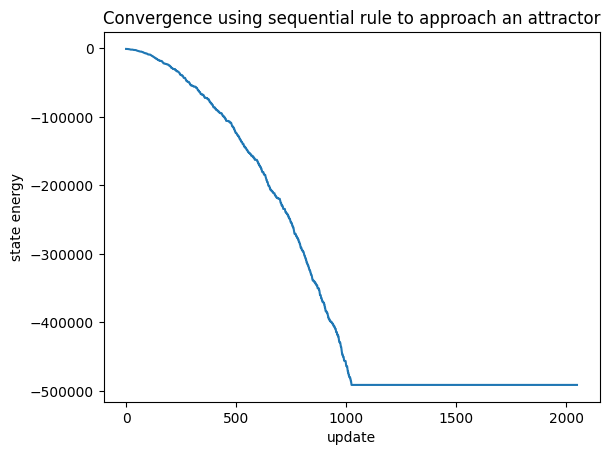
\includegraphics[width=.44\linewidth]{img/convergence_01.png}
    \caption{Convergence from a randomly generated pattern to an attractor}
    \label{fig:nrg_sconv_to_attr}
\end{figure}

\subsubsection{Random weight matrices}
\paragraph{Asymmetric case}
We studied the evolvement of the energy of the state of the model when initializing the matrix at random. Figure \ref{fig:nrg_rnd_weights_nsym} compares batch and sequential (1 epoch is 1024 updates) mode.

\begin{figure}[h]
    \centering
    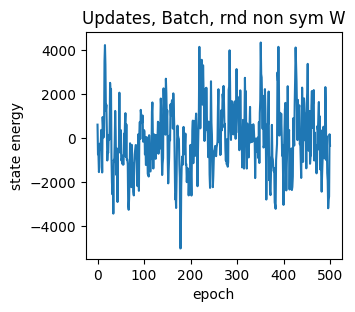
\includegraphics[width=.33\linewidth]{img/nrg_rand_w_non_sym_batch.png}
    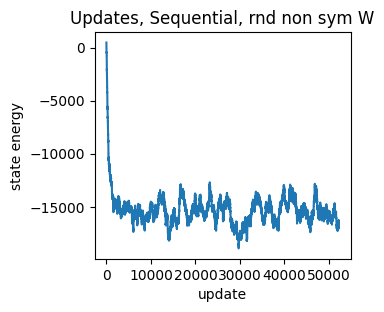
\includegraphics[width=.355\linewidth]{img/nrg_rand_w_non_sym_seq.png}
    \caption{Evolution of the energy of the state when initializing the weights as a random asymmetric matrix. Both models stopped by reaching a maximal number of iterations.}
    \label{fig:nrg_rnd_weights_nsym}
\end{figure}

In batch mode this is terrible, the energy bounces back and forth around 0, no convergence nor stabilization happens. In sequential a minimization occurs, but the system does not seem to be able to find a stable state. 

% It is possible that the randomness of the weight matrix creates very tiny local minimas. ?
% I dont think its necessarily the randomness, but rather because the scale of the weights is probably lower than in the usual case aka if the gauss used to init the weights has a bigger mean I would suspect the energy to be higher. In general case it is true that if you rescale all the weights by for example 2, the energy kindof doubles (>F.) 


\paragraph{Symmetric case}
By turning the weights to a symmetric matrix (i.e. $w=0.5*(w+w^\intercal)$), we can observe different results in Figure \ref{fig:nrg_rnd_weights_sym}. Both models are leading to a stabilization when performing updates. 
\begin{figure}[h]
    \centering
    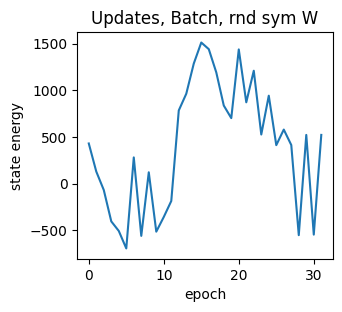
\includegraphics[width=.33\linewidth]{img/nrg_rand_w_sym_batch.png}
    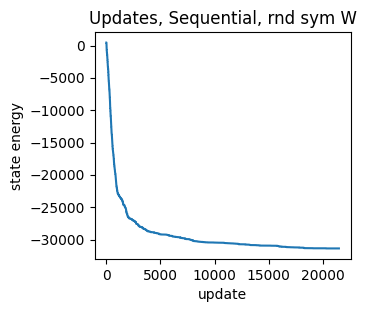
\includegraphics[width=.355\linewidth]{img/nrg_rand_w_sym_seq.png}
    \caption{Evolution of the energy of the state when initializing the weights as a random symmetric matrix. Both models stopped by stabilization.}
    \label{fig:nrg_rnd_weights_sym}
\end{figure}

However in batch mode, it leads to an oscillation between two states and its energy remains very close to 0 which is very high when compared to the stable state found by sequential update rule, which is around $-30000$ in this case.

The Observed difference between a converging symmetric and non-converging asymmetric weights matrix can be explain by the fact that the Hopfield network was designed to minimize energy values as defined by a symmetric matrix and the fact that the designed update rule is designed to accomplish that minimization. Using an asymmetric weights matrix breaks the first assumption needed to prove the convergence of a Hopfield network to a stable state.

\subsection{Distortion Resistance}

We added noise by flipping a certain percentage of the 3 learnt images and ran the network on this data to try to retrieve original pattern. Results (averaged over a few runs to make the curve smoother) are seen in Figure \ref{fig:dist_res}.

\begin{figure}[h]
    \centering
    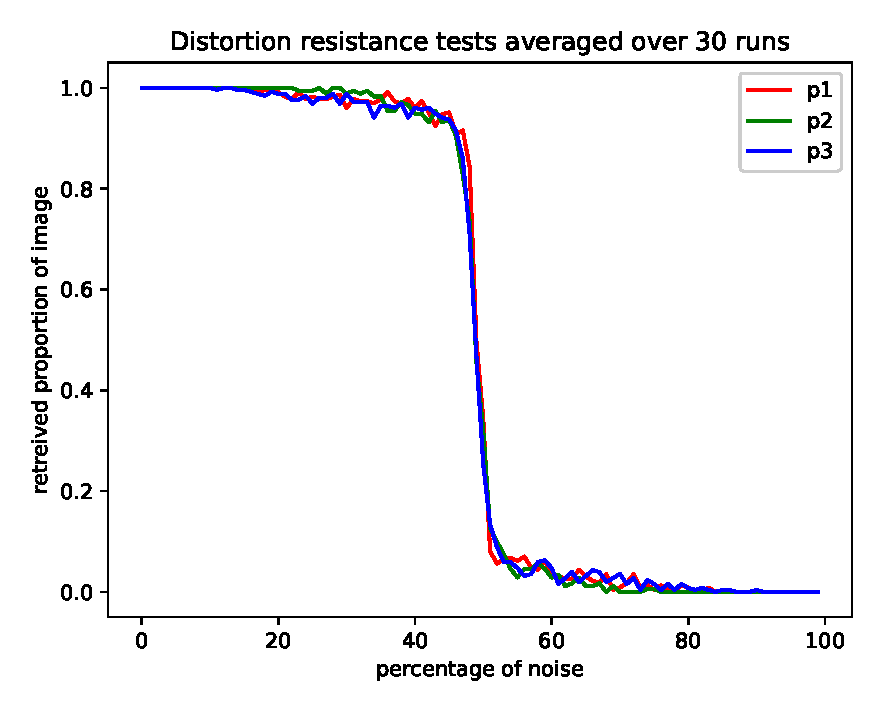
\includegraphics[width=.49\linewidth]{img/noise_distortion_01.eps}
    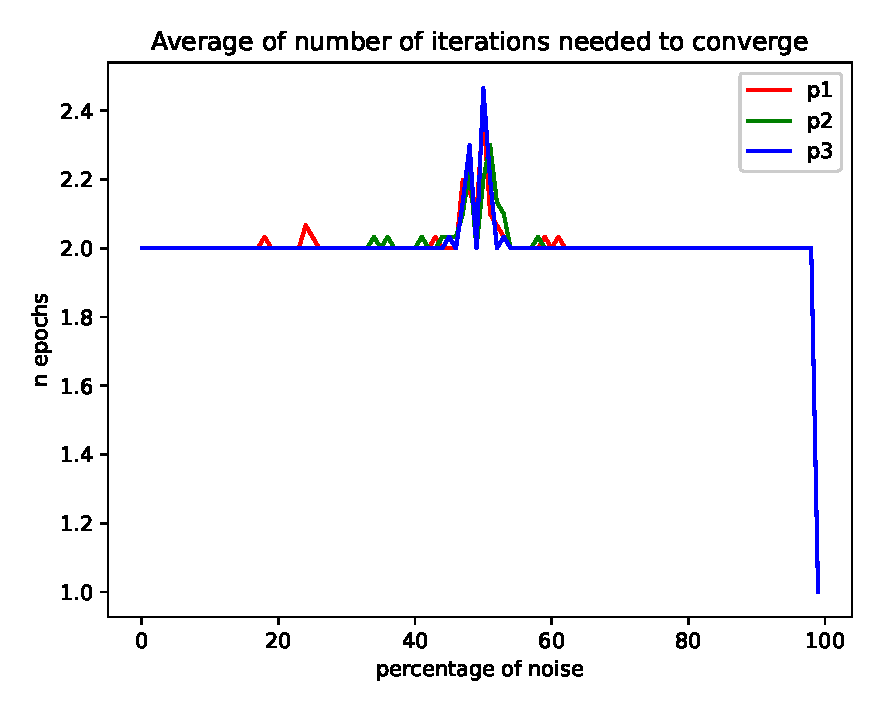
\includegraphics[width=.49\linewidth]{img/noise_distortion_02.eps}
    \caption{Performance of the network in respect to noise}
    \label{fig:dist_res}
\end{figure}

We did not observe any difference in the behaviour of the network according to the attractor that was being retrieved. Around 50\% of noise, there is a very steep downhill in the curve. After that point it is nearly impossible for the network to find the original pattern. However, before this point is reached, the network shows good capabilities for this task.

Except in the "grey zone" of around 50\% noise, the little model stabilizes in approximately 1 epoch, and even in the "grey zone" it just slightly goes up in average number of epochs. This shows that extra iterations did not help much in this case, the network would mostly stabilize in just one iteration. This observation can be explained by the fact that only three patterns are stored and not much of the networks capacity is yet used. As shown in Figure \ref{fig:nrg_att} we found another attractor (and its negative counterpart). After this noise threshold, the model tends to converge to another attractor than the pre-noise one.

The last scenario is at a noise level of 100\% (the pattern is fully flipped) and since the negative is also a stored pattern, it is also a stable local minima.

\subsection{Capacity}

In this task, we observed how adding more memories affected the stability of the network, using retrieval rate of non-distorted and moderately distorted patterns as a measure of the networks capacity.

Firstly we tried adding more memories to the initial three pictures (p1, p2 and p3) and observed that adding just one additional memory would prevent the network from converging to learnt patterns (Fig. \ref{fig:pic_vs_biased_random}), given either non-distorted or distorted images. Only first three patterns can be stored safely with perfect pattern retrieval, whereas for four patterns, the performance would abruptly drop to $0\%$ retrieval.

\begin{figure}[h]
    \centering
    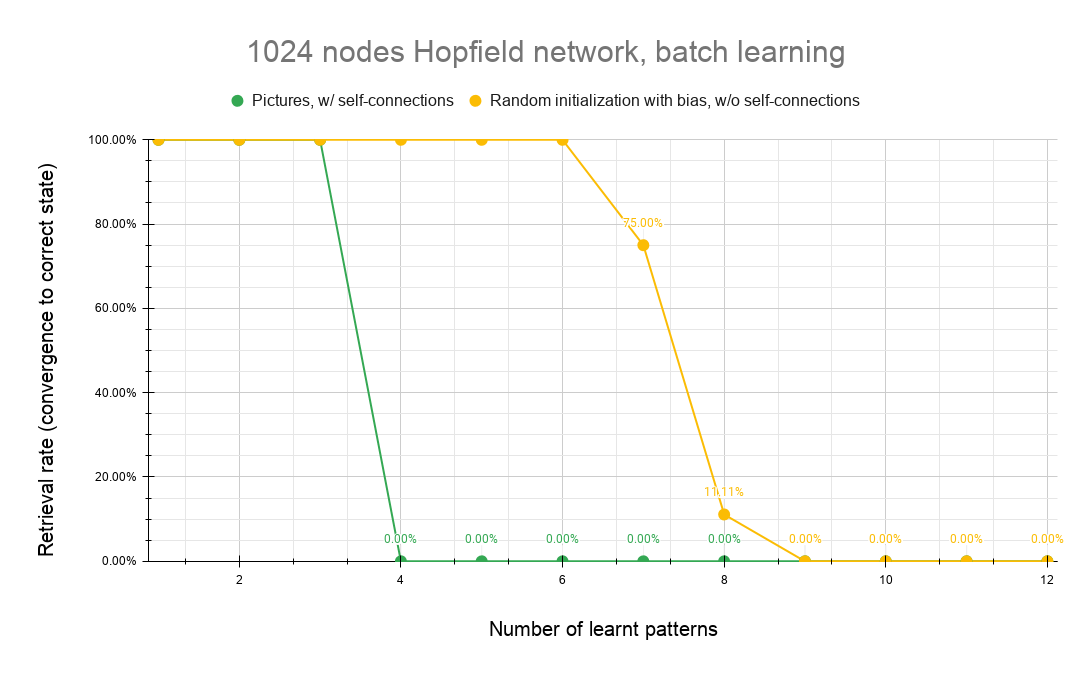
\includegraphics[width=0.8\linewidth]{img/6_pic_vs_biased_random.png}
    \caption{1024 nodes Hopfield network retrieval rate performance comparison for learning a handful of pictures and biased random vectors}
    \label{fig:pic_vs_biased_random}
\end{figure}

On the other hand, when using random vectors generated using $\mathcal{N}(0,\,1)\,$ (and then computing $sign()$) instead, we noticed enormous difference in performance metrics when adding more patterns to learn. The network could store up to $53$ patterns with perfect retrieval for patterns with distortions of maximal $20\%$ and up to $73$ patterns with retrieval higher than $90\%$ percent for patterns with up to the same amount of distortions, as shown in Figure \ref{fig:random_capacity}. Learning more patterns gradually decreases the performance, until after 200 learnt patterns when the retrieval rate is very low and approaches $0\%$. In Figure \ref{fig:random_capacity} one can also observe that the retrieval rate performance on non-distorted patterns is constantly higher that the performance on patterns with noise added. This difference in behaviour means lower robustness towards noise and higher noticeable degradation of basins of attraction.

\begin{figure}[h]
    \centering
    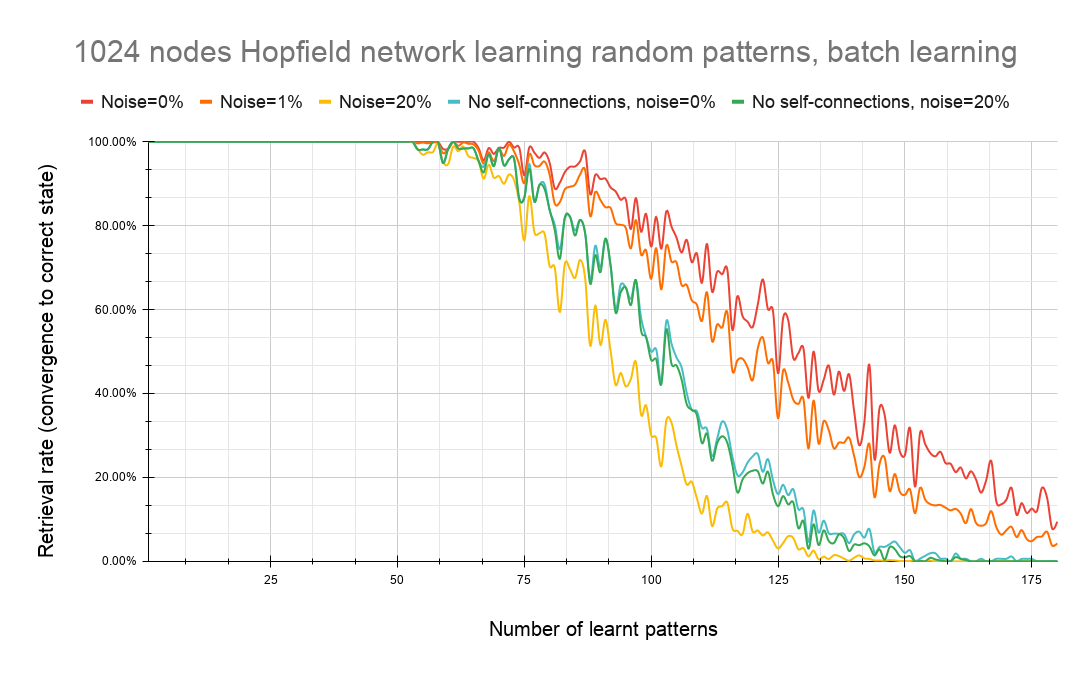
\includegraphics[width=\linewidth]{img/6_random_capacity.png}
    \caption{1024 nodes Hopfield network retrieval rate performance relation with different number of learnt patterns for learning random vectors with and without noise and self-connections. The cyan and green line overlap.}
    \label{fig:random_capacity}
\end{figure}

The huge difference in comparison with learning pictures can be explained by noting that the pictures are much more correlated than the randomly generated vectors.

In further investigation, we removed the self-connections $w_{ii}$ and observed that the difference between the curves from pure and noisy patterns, with up to $20\%$ of distortions, had no noticeable difference (Fig. \ref{fig:random_capacity}, cyan and green line overlap). Even though removing the self-connections seems to lower the memory performance (Fig. \ref{fig:random_capacity}, cyan and green line are below red and orange line), it is generally preferred not to have self-connections because they promote formation of spurious patterns and have a negative effect on noise removal capabilities. Having no self-connections results in higher noise robustness and thus more useful as well as more uniform basins of attraction, as can be seen in Figure \ref{fig:random_capacity} where the cyan and green line are above the yellow line.   

Additionally, we generated biased patterns with using $\mathcal{N}(0.5,\,1)\,$ instead of $\mathcal{N}(0,\,1)\,$, so the patterns had more 1's than -1's. The observed retrieval rate was drastically worse compared to the former case where no bias was used. The results were very similar to observed measures for pictures in that both had abrupt retrieval rate performance drop for less than $10$ learnt patterns. The similarity can be seen in Figure \ref{fig:pic_vs_biased_random}. % TBD Is this because sparse data is more correlated? Or should they rather be more easy to learn somehow beacause of sparsity?

\subsection{Sparse Patterns}
For our final subassignment we had to see how the network performed when learning sparse patterns, as well as observe the effect of adding constant bias. For testing we used a 100-neuron network and, ipso facto, 100-dimensional patterns. The learning and update rule were modified as specified in the subassignment in order to achieve a \{0, 1\} binary output (as opposed to the \{-1, 1\} used before). In what follows, we describe only the observations we made, but we were not able to draw conclusions or base the results on intuitive basis.

With self-connections, learning patterns with an activity of 10\% for different bias ($\theta$) values resulted in various results. The network performed best using $\theta = 0.3$ and could store up to 25 sparse patterns. This is a large number in relation to the dimensionality of the network.

For a lower bias of around $\theta = 0.05$ if the network is given too many patterns it saturates and becomes stable in all states (the diagonal becomes the strongest part of the weight matrix), allowing it to learn any amount of patterns, but rendering it useless. Using a larger bias like the aforementioned $\theta = 0.3$ doesn't allow this to happen as the bias drags everything into 0 (Figure \ref{fig:saturation}).

\begin{figure}[h]
    \centering
    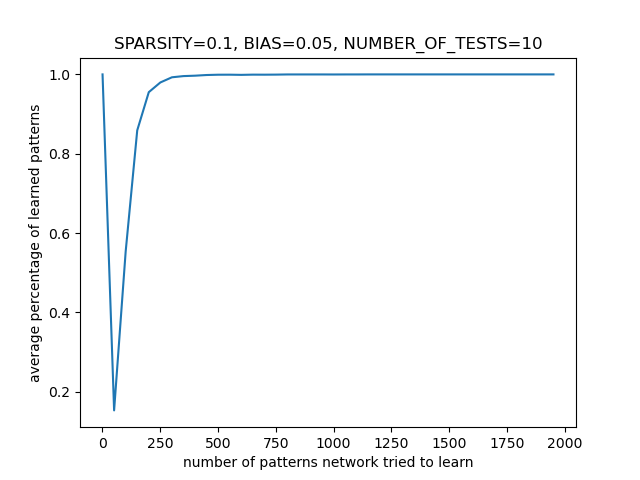
\includegraphics[width=.49\linewidth]{img/sparsity=0.1_bias=0.05000.png}
    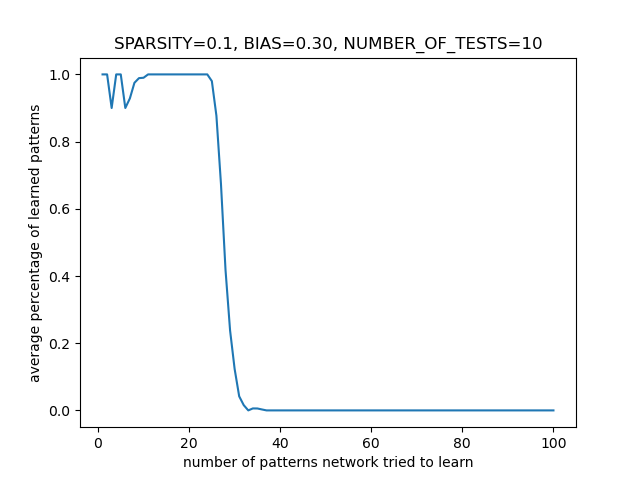
\includegraphics[width=.49\linewidth]{img/sparsity=0.1_bias=0.30000.png}
    \caption{Percentage of learned patterns vs. number of patterns network tried to learn for $\theta = 0.05$ and $\theta = 0.3$}
    \label{fig:saturation}
\end{figure}

Without self-connections the network could reliably learn up to 10 10\% patterns, 6 5\% patterns, and about 100 1\% patterns. If we add any bias to the 1\% pattern network it drags everything into 0 making the network useless.

\section{Final remarks}
This assignment was an interesting insight into the workings of Hebbian networks. It was slightly easier than the first two labs, but since the tasks were quite sequential in relation one to another it was hard to split the work between team members efficiently. 

\end{document}
